\documentclass{article}

% if you need to pass options to natbib, use, e.g.:
% \PassOptionsToPackage{numbers, compress}{natbib}
% before loading nips_2016
%
% to avoid loading the natbib package, add option nonatbib:
% \usepackage[nonatbib]{nips_2016}

\usepackage{nips2016}
%\usepackage[final]{nips_2016}

\usepackage[utf8]{inputenc} % allow utf-8 input
\usepackage[T1]{fontenc}    % use 8-bit T1 fonts
\usepackage{hyperref}       % hyperlinks
\usepackage{url}            % simple URL typesetting
\usepackage{booktabs}       % professional-quality tables
\usepackage{amsfonts}       % blackboard math symbols
\usepackage{amssymb}
\usepackage{nicefrac}       % compact symbols for 1/2, etc.
\usepackage{microtype}      % microtypography
\usepackage{subfigure}
\usepackage{graphicx}
\usepackage{setspace}
\usepackage{color}



\title{Convolutional Neural Networks on Graphs\\ with Fast Localized Spectral Filtering}

% The \author macro works with any number of authors. There are two
% commands used to separate the names and addresses of multiple
% authors: \And and \AND.
%
% Using \And between authors leaves it to LaTeX to determine where to
% break the lines. Using \AND forces a line break at that point. So,
% if LaTeX puts 3 of 4 authors names on the first line, and the last
% on the second line, try using \AND instead of \And before the third
% author name.

\author{
  Michaël Defferrard \\ %\thanks{further info} \\
  %Department of Electrical Engineering \\
  %École Polytechnique Fédérale de Lausanne (EPFL) \\
  EPFL \\
  Lausanne, Switzerland \\
  \texttt{michael.defferrard@epfl.ch} \\
  \And % \AND
  Xavier Bresson \\
  EPFL \\
  Lausanne, Switzerland \\
  \texttt{xavier.bresson@epfl.ch} \\
  \And
  Pierre Vandergheynst \\
  EPFL \\
  Lausanne, Switzerland \\
  \texttt{pierre.vandergheynst@epfl.ch} \\
}

\usepackage[acronym]{glossaries}
\newacronym{SVD}{SVD}{Singular Value Decomposition}
\newacronym{SGD}{SGD}{Stochastic Gradient Descent}
\newacronym{PSD}{PSD}{positive semidefinite}

\DeclareMathOperator*{\diag}{diag}
\DeclareMathOperator*{\argmin}{arg\,min}
\DeclareMathOperator*{\spn}{span}
\renewcommand{\L}{\mathcal{L}}
\newcommand{\G}{\mathcal{G}}
\renewcommand{\H}{\mathcal{H}}
\newcommand{\K}{\mathcal{K}}
\newcommand{\V}{\mathcal{V}}
\newcommand{\E}{\mathcal{E}}
\newcommand{\W}{\mathcal{W}}
\newcommand{\R}{\mathbb{R}}
\newcommand{\N}{\mathbb{N}}
\newcommand{\Xh}{\hat{X}}
\newcommand{\Yh}{\hat{Y}}
\newcommand{\st}{\ \text{s.t.} \,}
\newcommand{\norm}[1]{\left\| #1 \right\|}

\begin{document}
% \nipsfinalcopy is no longer used

\maketitle



\begin{abstract}
Convolutional neural networks have greatly improved state-of-the-art performances in computer vision and speech analysis tasks, due to its high ability to extract multiple levels of representations of data. In this work, we are interested in generalizing convolutional neural networks from low-dimensional regular grids, where image, video and speech are represented, to high-dimensional irregular domains, such as social networks, biological graphs like gene regulatory and brain connectivity networks, telecommunication networks, or words' embedding. We present a formulation of convolutional neural networks on graphs in the context of the emerging field of signal processing on graphs, which provides the necessary mathematical background and efficient numerical schemes to design fast localized convolutional filters on graphs. Numerical experiments on MNIST and 20NEWS demonstrate the ability of the system to learn local stationary features on graphs, as long as the graph is well-constructed.
\end{abstract}

%Previous works have been developed along this today essential line of research, but they lack of mathematical foundations and efficient learning of filters.




\begin{figure}[h!]
\centering
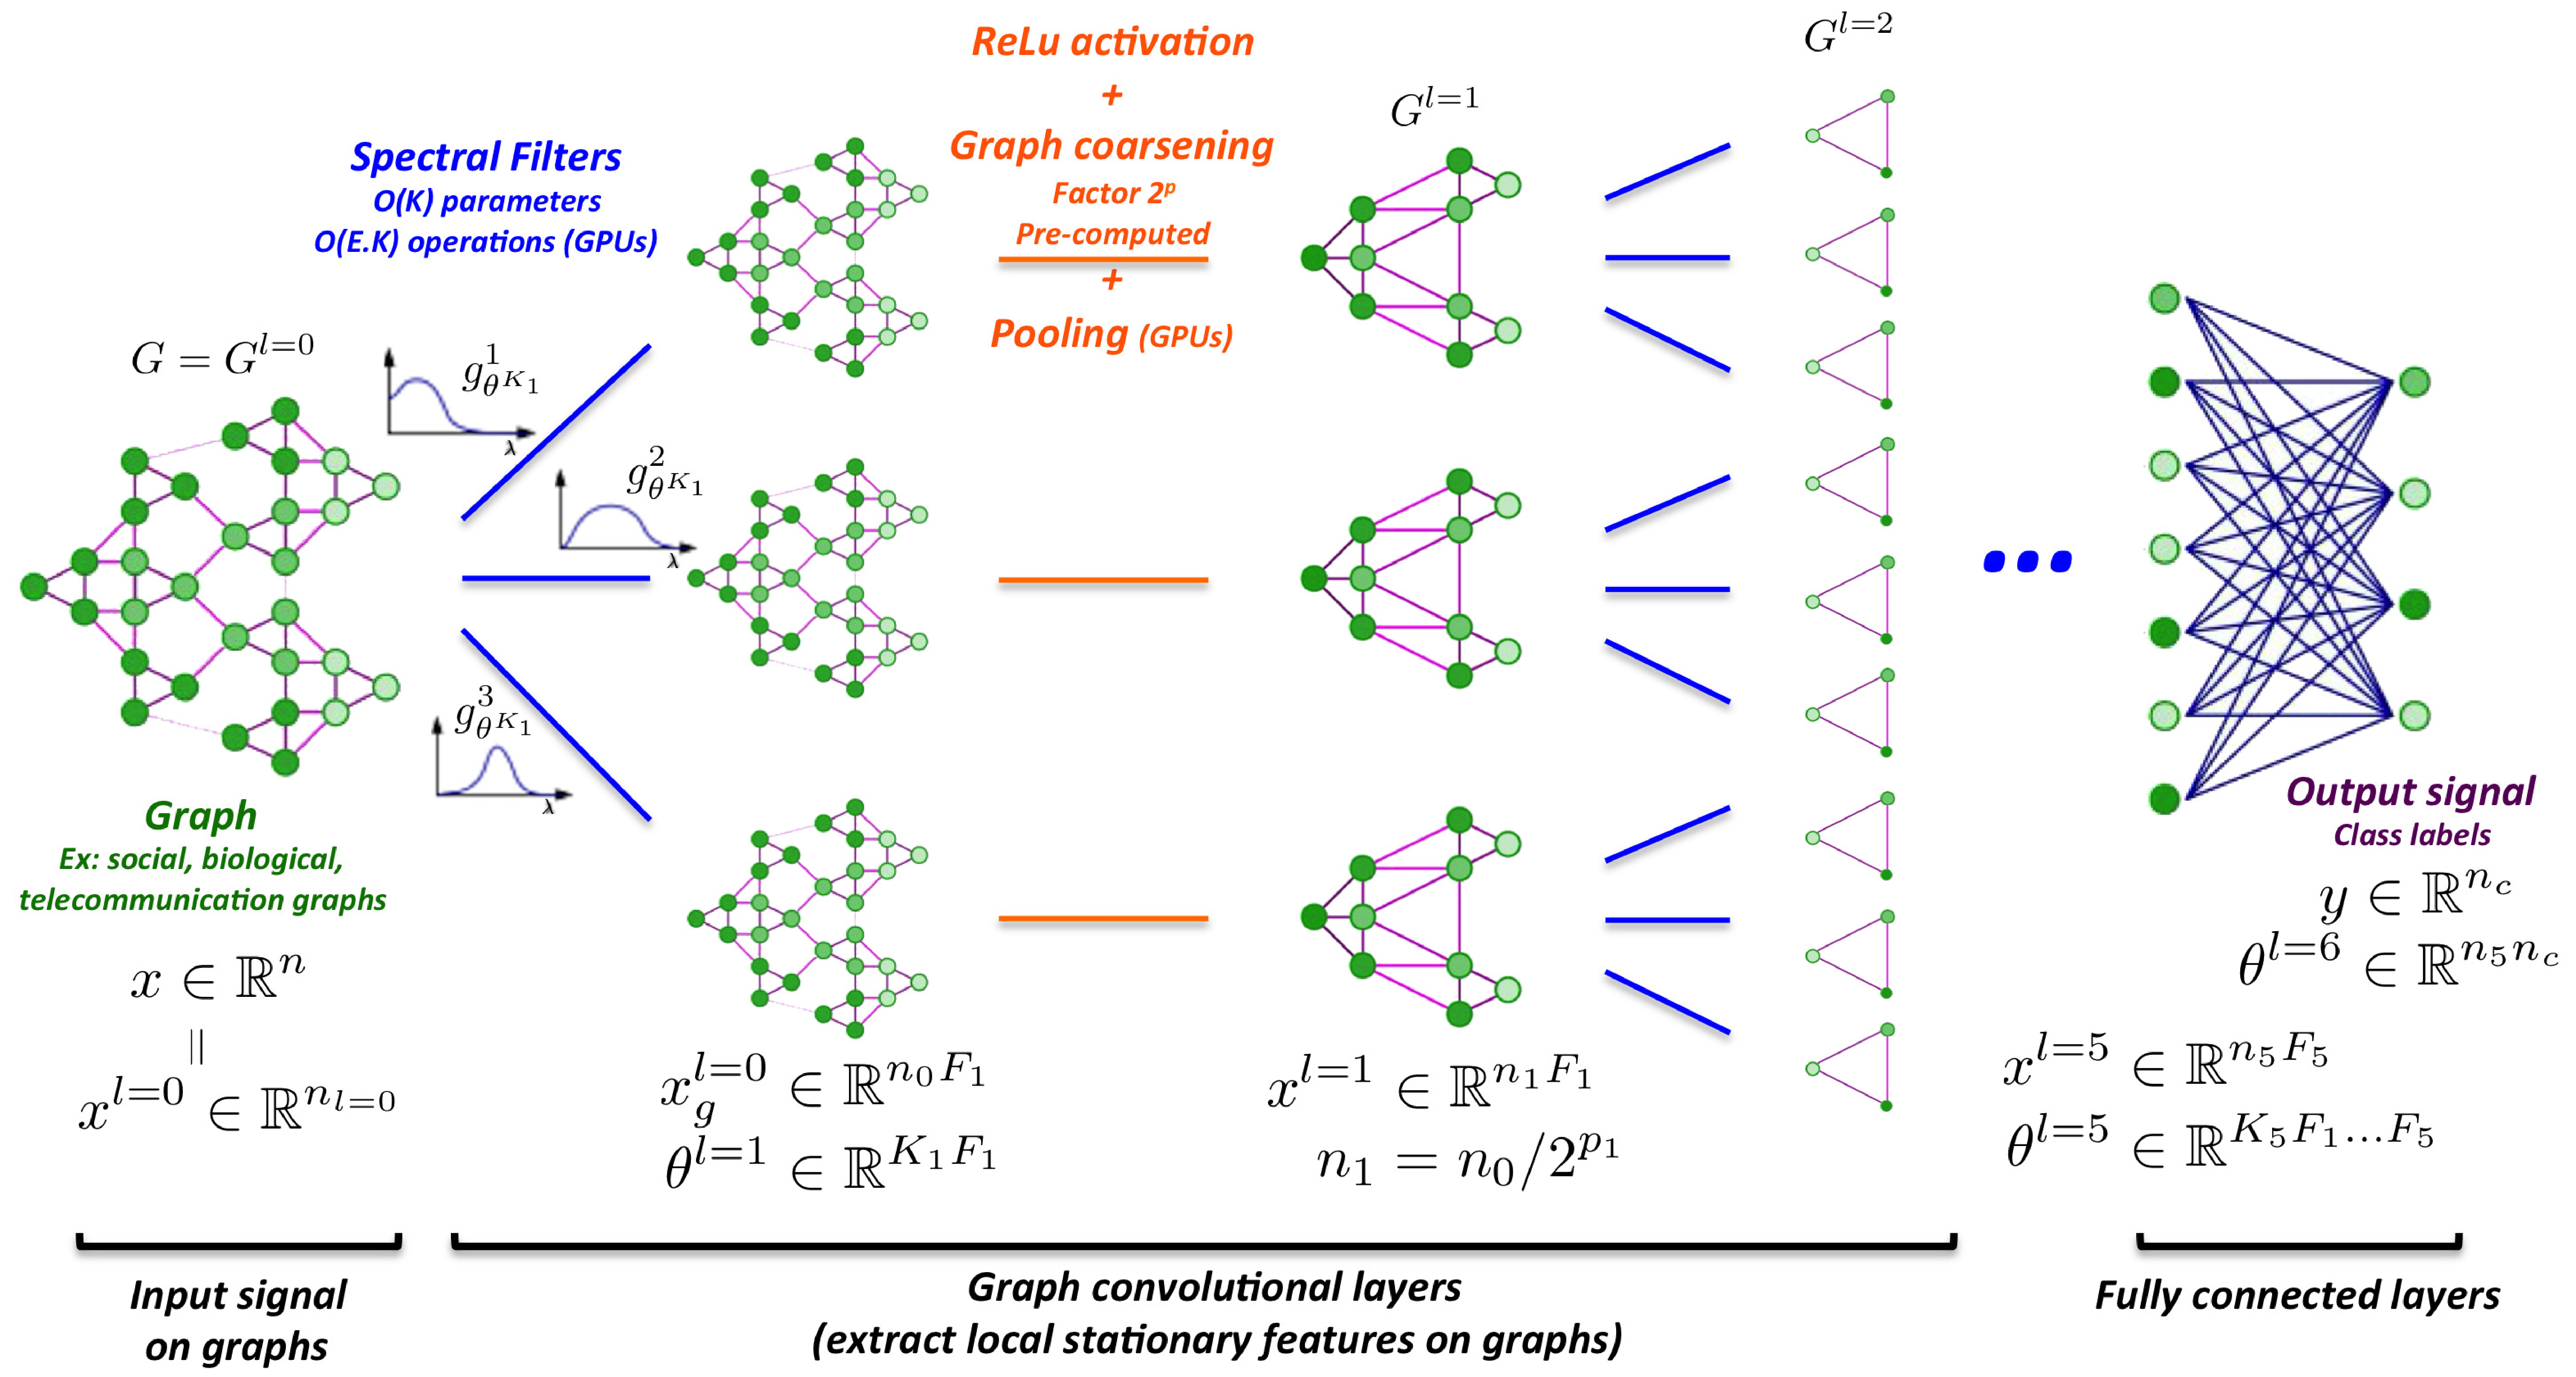
\includegraphics[width=13.5cm]{images/illustrationCNNgraphs.eps}
%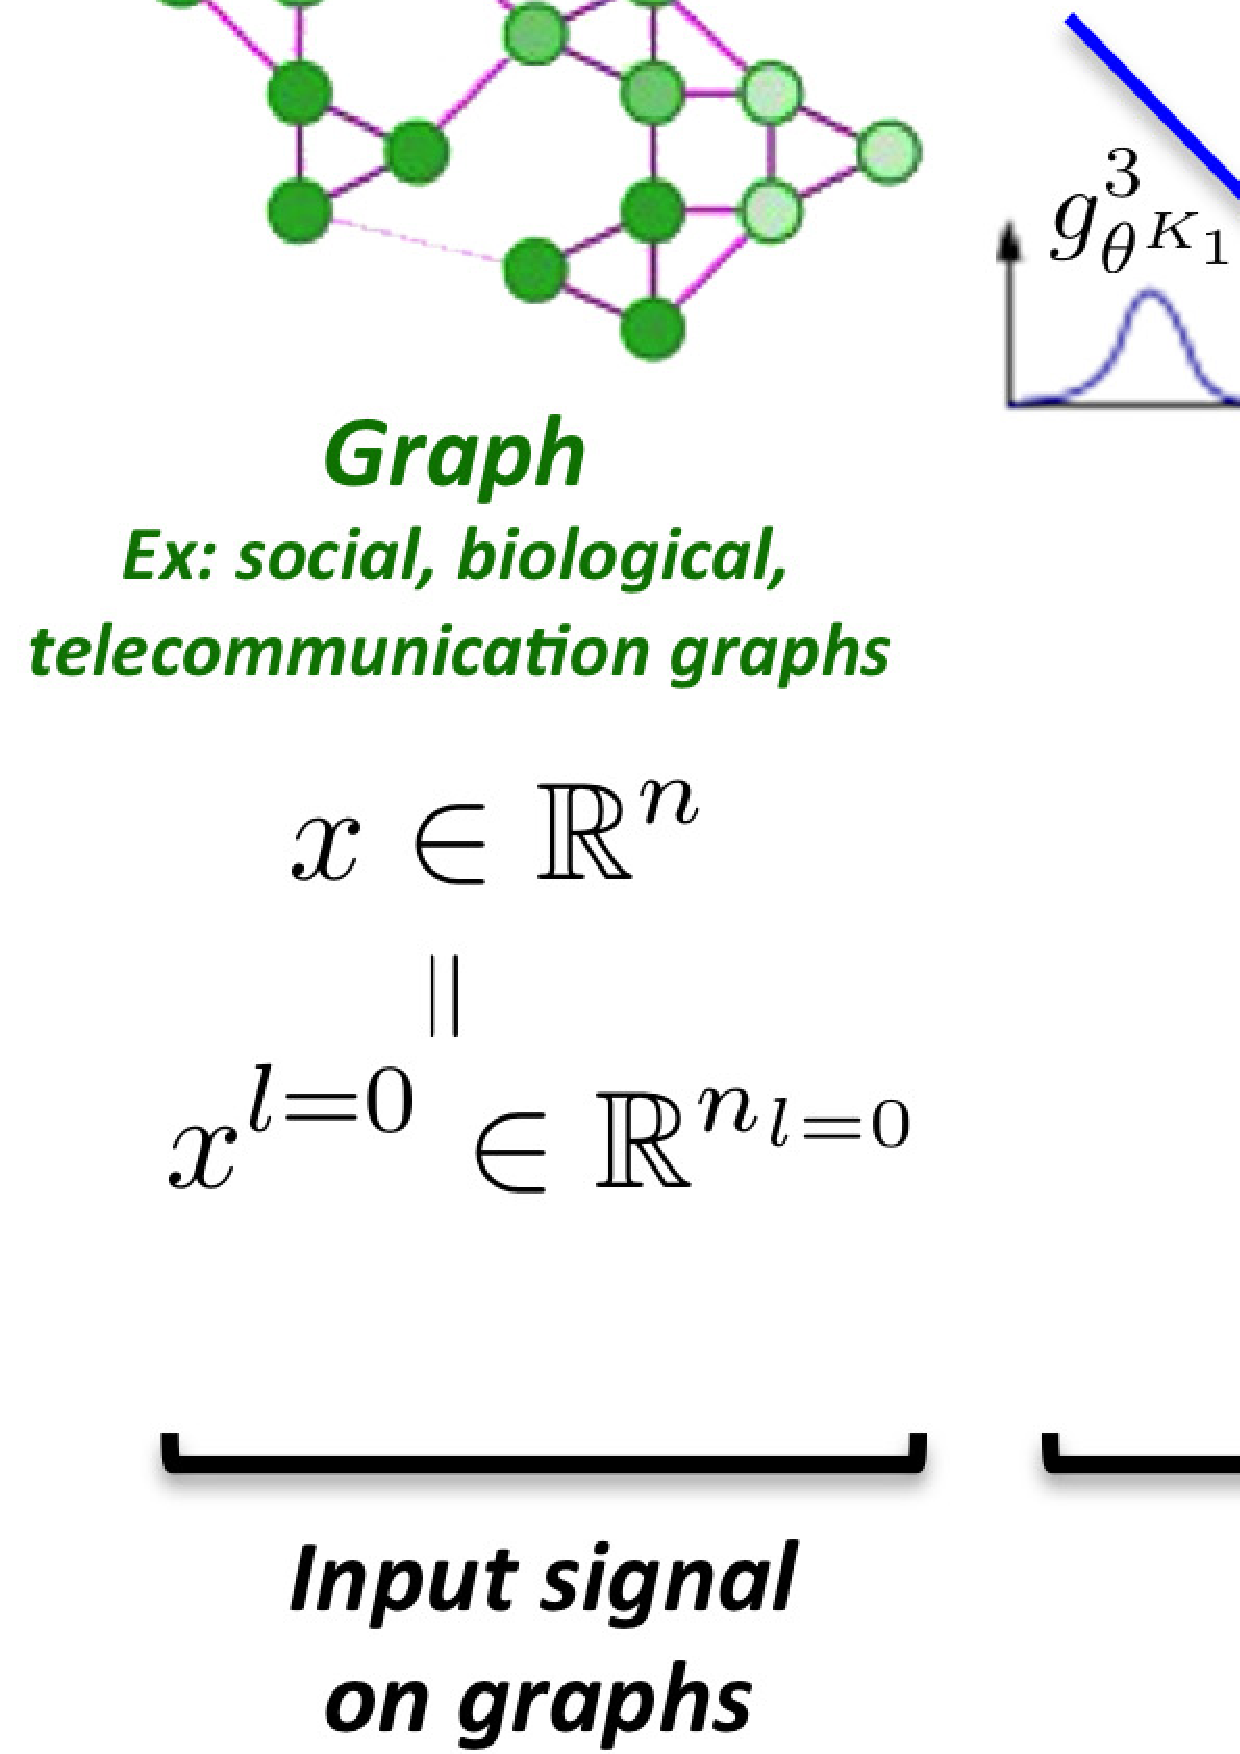
\includegraphics[width=13.5cm]{images/illustrationCNNgraphs.png}
\caption{Architecture of the proposed CNNs on graphs. Notation: $l$ is the coarsening level, $x^l$ are the downsampled signals at layer $l$, $G^l$ is the coarser graph, $g_{\theta^{K_l}}$ are the spectral filters at layer $l$, $x_g^l$ are the filtered signals, $p_l$ is the coarsening exponent, $n_c$ is the number of classes, $y$ is the output signal, and $\theta^l$ is the number of parameters to learn at $l$.}
\label{fig:}
\end{figure}







\section{Introduction}
\vspace{-0.2cm}
Convolutional neural networks (CNNs) \cite{pro:LeCunBottouBengioHaffner98MNIST} offer an efficient architecture to extract highly meaningful statistical patterns in large-scale and high-dimensional datasets. The key success of CNNs is its advanced ability to learn local stationary structures and compose them to form multi-scale hierarchical patterns. Precisely, CNNs extract the local stationarity property of the input data or signals by revealing local features that are shared across the data domain. These similar features are identified with localized convolutional filters or kernels, which are learned from the data. Convolutional filters are shift- or translation-invariant filters, meaning they are able to recognize identical features independently of their spatial locations. Localized kernels or compactly supported filters refer to filters that extract local features independently of the input data size, with a support size that can be much smaller than the input size. \\
The compositional local stationarity property of CNNs can be efficiently implemented on regular grids, like image and sound domains, as convolutional and downsampling operators are mathematically well-defined on such discretized Euclidean spaces. This has led to the breakthrough of CNNs in image, video, and sound recognition tasks \cite{art:LeCunBengioHinton15DL} as these data lie on low-dimensional regular lattices. But not all data lie on regular grids. User data on social networks, gene data on biological regulatory networks, log data on telecommunication networks, or text documents on words' embedding are important examples of data lying on irregular or non-Euclidean domains. Unfortunately, CNNs cannot be directly applied to such complex domains.\\
A generalization of CNNs to irregular grids is not direct as the basic convolutional and downsampling operators, necessary to extract compositional local stationarity features, are not mathematically clear on these domains. This makes this extension mathematically challenging, both in theory and in implementation. The goal of this work is to leverage the recent works of \cite{pro:GregorLeCun10LRF,pro:CoatesNg11LRF,art:BrunaZarembaSzlamLeCun13DLgraphs,art:HenaffBrunaLeCun15DLgraphs,art:HammondVandergheynstGribonval11GraphWav,art:ShumanNarangFrossardOrtegaVandergheynst13ReviewSPG,art:ShumanRicaudVandergheynst16Local} to introduce an efficient implementation of CNNs on irregular domains represented here as graphs. Graphs are universal representations of heterogeneous pairwise relationships between possibly high-dimensional data. Graphs can encode complex geometric structures, and can be studied with strong mathematical tools such as graph spectral theory, a blend between graph theory and harmonic analysis.\\
The major bottleneck of generalizing CNNs to graphs is the design of fast and localized filters on graphs, that are the core elements to extract local stationarity structures. Our major goal is to overcome this barrier. We will make use of recent tools developed in the context of signal processing on graphs (SPG) \cite{art:ShumanNarangFrossardOrtegaVandergheynst13ReviewSPG} to precisely control the spatial support of graph filters using the so-called polynomial kernel localization \cite{art:ShumanRicaudVandergheynst16Local}, and to perform an efficient backward propagation technique using the Chebyshev technique \cite{art:HenaffBrunaLeCun15DLgraphs}. Eventually, a generic and efficient implementation of CNNs on graphs may pave the way to the development of a potentially large class of deep learning techniques for graph-based data. 
  


\section{Related Works}
\vspace{-0.2cm}
{\bf CNNs on non-Euclidean domains.} Extending the success of CNNs to non-Euclidean domains is essential to boost the power analysis of data lying on complex networks like biological, social or telecommunication networks. This is a recent line of works, with a preliminary approach coming from the local reception fields in \cite{pro:GregorLeCun10LRF,pro:CoatesNg11LRF}, and applied successfully to object recognition in computer vision. The main idea is to unsupervisedly learn groups of similar features. This is highly useful to automatically choose a limited number of connections between two successive layers. This approach is however not able to extract similar groups over the data domain, as it is not clear how to define convolutional filters on these groups.  \\
In \cite{art:BrunaZarembaSzlamLeCun13DLgraphs,art:HenaffBrunaLeCun15DLgraphs}, the authors proposed a generalization of CNNs on graphs using graph counterparts of grid convolution and downsampling. They were able to learn shift-invariant or convolutional filters on graphs using the convolution theorem \cite{book:Mallat99wavelets} that defines convolutional operators as linear operators that diagonalize in the Fourier basis (represented by the eigenvectors of the Laplacian operator). They also designed a strategy to learn the graph structure from the data, and apply their model on image recognition, text categorization and bioinformatics. This promising approach is however limited in implementation as forward and backward evaluations have complexity $O(n^2)$ due to the matrix multiplication operations that operate the graph Fourier transforms. Besides, there is no strong control over the support size of the convolutional kernels, which is essential to design localized filters to extract local stationary features, independent of the input size. \\
The authors in \cite{pro:MasciBoscainiBronsteinVandergheynst15GeoDL,art:MasciBoscainiBronsteinVandergheynst15ShapeNet} introduced ShapeNet, a generalization of CNNs to 3D-meshes, a class of smooth low-dimensional non-Euclidean spaces. They used geodesic polar coordinates to define mesh patches and formulated a deep learning architecture. They obtained state-of-the-art results for shape recognition tasks.\\
Finally, the papers \cite{pro:ChenChengMallat14deepHaar,pro:RustamovGuibas14deepHaar} investigated the construction Haar wavelet transforms on graphs using a deep hierarchical architecture. They applied these deep wavelets on graphs to object recognition on sphere, and to sparse reconstruction of faces. \\
{\bf Signal Processing on Graphs.} SPG is an emerging field that aims at bridging the gap between signal processing techniques like wavelet analysis and graph theory such as spectral graph analysis \cite{art:BelkinNiyogi05LaplaBeltrami,art:VonLuxburg07Tutorial}. The main goal is to generalize fundamental analysis operations for signals from regular grids to irregular structures embodying by graphs. We refer the reader to \cite{art:ShumanNarangFrossardOrtegaVandergheynst13ReviewSPG} for an introduction of the field. Standard operations on grids such as convolution, translation, filtering, dilatation, modulation, downsampling do not extend directly to graphs and thus require new mathematical definitions while keeping the original intuitive concepts. In this context, the authors of \cite{art:HammondVandergheynstGribonval11GraphWav,art:CoifmanLafon06DifMap,pro:GavishNadlerCoifman10GraphHaar} revisited the construction of wavelet operators on graphs. In \cite{art:ShumanFarajiVandergheynst16PyramTrans,art:RamEladCohen11TreeWavelets}, the authors designed a technique to perform mutli-scale pyramid transforms on graphs. The works of \cite{pro:TsitsveroBarbarossa15Uncert,pro:PasdeloupAlamiGriponRabbat15Uncert,art:PerraudinRicaudShumanVandergheynst16Uncert} redefined uncertainty principles on graphs, and showed that intuitive concepts may be lost, but can also produce enhanced localization principles for signals on graphs. In \cite{pro:HammondRaoaroorJacquesVandergheynst10LassoGraWav}, it was shown how to carry out lasso-based signal regularization on graphs, and studied the intertwined relationships between smoothness and sparsity on graphs. In \cite{pro:TremblayPuyGribonvalVandergheynst16CompSpecClus}, the authors investigated compressed sensing recovery conditions for graph spectral signal analysis. \\
Beyond this work, our long-term goal is to make use of SPG tools as much as possible to formulate mathematically well-designed techniques of CNNs on graphs. This paper introduces the mathematical and computational foundations of such models, while future developments may consider enhanced graph filters like graph wavelet operators, spectral graph coarsening techniques, and improved localization properties.




\section{Contributions}
\vspace{-0.2cm}
{\textbf {\textit {(1)}}} Learning deep fully connected networks is almost computationally untractable for large data domain. Fortunately, for data satisfying stationarity and hierarchical compositionality structure, CNNs have proven to be remarkably powerful to identify highly informative features using low learning complexity. For example, learning a single layer with $n$ input coordinates and $m<n$ outputs require $O(n^2)$ complexity to learn fully connected networks. It also requires the complexity $O(n)$ to learn any arbitrary filter, and $O(S)$ for localized filters, where $S$ is the size of the filter support, independent of the input size $n$. One of our main contributions is to stay with the same low complexity for learning graph convolutional filters. We will show it is actually possible to keep exactly the same complexity as standard CNNs, i.e. $O(S)$ for localized graph filters.\\
{\textbf {\textit {(2)}}} The backpropagation learning algorithm requires to run convolutional operations, which can be efficiently implemented by FFT on grids with complexity $O(n\log n)$. Convolution on graphs can also be implemented by matrix multiplications representing the forward and backward graph Fourier transforms, but it is expensive as the complexity is $O(n^2)$. As noticed in \cite{art:HenaffBrunaLeCun15DLgraphs}, this complexity is a strong bottleneck to deal with large-scale problems. We will greatly improve this complexity by reducing to $O(E.S)$, where $E$ is the number of edges in the given graph, using the Chebyshev technique from SPG \cite{art:ShumanNarangFrossardOrtegaVandergheynst13ReviewSPG}. Besides, as most real-world graphs are highly sparse, we have $E\ll n^2$, and therefore a low complexity for the matrix multiplication operations. Eventually, the Chebyshev computations can be naturally distributed on GPUs, as we did in our experiments.\\
{\textbf {\textit {(3)}}} We introduce an efficient pooling strategy for CNNs on graphs, that also makes use of distributed computing architecture like GPUs. The pooling approach consists on two stages. First, a graph coarsening procedure based on METIS \cite{art:DhillonGuanKulis07Graclus,art:KarypisKumar98Metis} is successively applied to the original graph to produce coarser versions of the graph. Second, at each coarsening level, we sequentially order all nodes such that two successive indexed nodes are the parent nodes of the child node in the next coarser level. This node indexation structure in memory satisfies parallel architectures. \\
{\textbf {\textit {(4)}}} We regard this proposed work as the funding paper that bridges the gap between two powerful fields, namely deep learning and signal processing on graphs. In the future, we expect to further benefit from tools in SPG to enhance the formulation of CNNs on graphs. \\
{\textbf {\textit {(5)}}} We revisit the Euclidean case in the numerical experiments with the standard MNIST image classification problem. The model is able to learn localized convolutional filters and achieve 98.65\% of success rate. More interestingly, we apply our model to the text categorization problem on 20NEWS. We also demonstrate that our techniques is able to extract local stationary features, as it improves by 2.5\% the classification accuracy when no convolutional are present. We observe that the quality of the graph construction is strongly linked to the quality of the convolutional layers. Finally, we demonstrate the computational performance of our model over \cite{art:HenaffBrunaLeCun15DLgraphs}.



\section{Learning Localized Graph Filters}
\vspace{-0.2cm}
In this section, we explore how to design efficient localized convolutional filters on graphs.



\subsection{Signal Processing on Graphs and Localized Filters}
\vspace{-0.2cm}
{\bf Graph Fourier Transform.} We are interested in processing signals defined on undirected and connected graphs $G=(V,E,W)$, where $V$ is the set of vertices with $|V|=n$, $E$ is the set of edges and $W$ is the weighted adjacency matrix encoding the connection weights between two vertices. A signal $x:V\rightarrow\mathbb{R}$ defined on the nodes of the graph may be regarded as a vector $x\in\mathbb{R}^n$ where $x_i$ is the value of $x$ at the $i^{th}$ node. An essential operator in spectral graph analysis is the graph Laplacian \cite{book:Chung97Spectral}, which unnormalized definition is $L=D-W\in\mathbb{R}^{n\times n}$ with $D\in\mathbb{R}^{n\times n}$ is the diagonal degree matrix where $D_{ii}=\sum_jW_{ij}$, and its normalized definition is $L=I_n-D^{-1/2}WD^{-1/2}$ where $I_n$ is the identity matrix. As $L$ is a real symmetric positive semidefinite matrix, it has a complete set of orthonormal eigenvectors $\{u_l\}_{l=0}^{n-1}\in\mathbb{R}^n$, known as the graph Fourier modes, and their associated real nonnegative eigenvalues $\{\lambda_l\}_{l=0}^{n-1}$, which are the frequencies of the graph system. Equivalently, linear operator $L$ diagonalizes the Fourier basis matrix $U=[u_0,...,u_{n-1}]\in\mathbb{R}^{n\times n}$ such that $L=U\Lambda U^T$ where $\Lambda=\diag(\lambda_l)$. We can now define the graph Fourier transform (GFT) and its inverse \cite{art:ShumanNarangFrossardOrtegaVandergheynst13ReviewSPG}. The GFT of a spatial signal $x\in\mathbb{R}^n$ is $\hat{x}=U^Tx\in\mathbb{R}^n$, and the inverse GFT is $x=U\hat{x}$. Using GFT we can now generate fundamental operations of signal processing on graphs such as convolution and filtering. \\
{\bf Convolutional Filters.} The graph convolutional operator is simply defined in the Fourier space such as $f\ast_G g=U((U^Tf) \odot (U^Tg))$, where $\odot$ the element-wise Hadamard product. Then the convolutional filtering operation on graphs is defined as $y=g_\theta(L)x\in\mathbb{R}^n$, where $g_\theta(L)=g_\theta(U\Lambda U^T)=Ug_\theta(\Lambda) U^T\in\mathbb{R}^{n\times n}$ where $g_\theta(\Lambda)=\diag(\theta)$ and $\theta\in\mathbb{R}^n$ is the filter expressed in the Fourier space. Remember that convolutional filters, i.e. translation-invariant filters on graphs, can only be defined in the Fourier domain as convolution operators are not defined in the vertex space. \\
{\bf Localized Convolutional Filters.} Learning convolutional filters on graphs boils down to learn spectral multipliers $\theta$ of complexity $O(n)$, the size of the input data. Our goal is to reduce this complexity to $O(S)$, the support size of the filter in the vertex space, exactly as in standard CNNs. For this, we will make use of a property called polynomial localization \cite{art:ShumanRicaudVandergheynst16Local}. Let us represent $\theta=\{\theta_{\{{\lambda_l}\}_{l=0}^n}\}\in\mathbb{R}^n$ as a $K$-th differentiable polynomial function: $\theta_{\lambda_l}^K(a)=\sum_{k=0}^{k-1}a_k \lambda_l^k$, where $a=\{a_k\}_{k=0}^{K-1}\in\mathbb{R}^K$. The polynomial localization theorem \cite{art:ShumanRicaudVandergheynst16Local} shows that $(T_ig_{\theta^K})_j=(\delta_i \ast_G (Ug_{\theta^K}))_j=0$ for $d_G(i,j)>K$ where $d_G$ is the shortest distance on graph, meaning that the support of the associated spatial filter is exactly $K$-localized, all values are zero after $K$ hopes. Consequently, spectral filters represented by $K$-order polynomials are spatially localized with support $S=K$, implying the low learning complexity $O(K)$ for each filter. We notice that the authors \cite{art:HenaffBrunaLeCun15DLgraphs} also used a $K$-order polynomials represented by splines, but they did not formalize the quantitive relationship between filter support size and polynomial order. Finally, it is also possible to estimate the spatial decaying profile of the filter \cite{art:ShumanRicaudVandergheynst16Local}: for any K-localized filter centered at vertex $i$, we have the profile $|(T_ig_{\theta^K})(j)|\leq\big[\frac{2\sqrt{n}}{K!}(\frac{\lambda_{max}}{4})^K \sup_{\lambda}|(Ug_{\theta^K})^K(\lambda)|\big]$, which may be useful for graph filter analysis. 





\subsection{Fast Filter Learning with Chebyshev Technique}
\vspace{-0.2cm}
Let $y$ be a signal $x$ filtered on the graph: $y=g_\theta(L)x=U(g_\theta(\Lambda) (U^Tx))$. Learning a spectral filter can be reduced to a complexity $O(K)$ by polynomial parametrization. However, the numerical computation of $y$ still requires two full matrix multiplications by $U^T,U$ with a high complexity of $O(n^2)$, and these matrix multiplications must be done several times in the backpropagation process. This is a computational bottleneck, identified in \cite{art:HenaffBrunaLeCun15DLgraphs}, with an additional cost of $O(n^3)$ for computing a full eigenvalue decomposition of $L$ to get $U$. We can overcome this computational issue using a Chebyshev technique as proposed in SPG \cite{art:HammondVandergheynstGribonval11GraphWav}. We will also explore in the future the Lanczos technique \cite{art:SusnjaraPerraudinKressnerVandergheynst15Lanczos}, which seems attractive because of the independence of the coefficients. \\
We first recall the fundamental recurrence property of Chebyshev polynomials. Let the Chebyshev polynomial \(T_k(x)\) of order \(k\) be generated by the recurrence relation \(T_k(x) = 2x T_{k-1}(x) - T_{k-2}(x)\) with \(T_0 = 1\) and
\(T_1 = x\). These polynomials form an orthogonal basis. Then, the K-compact spectral filter $g_{\theta^K}(\Lambda)$ can be defined as $g_{\theta^K}(\Lambda)=\sum_{k=0}^{K-1}\theta_k T_k(\tilde{\Lambda})$ of order \(k\) evaluated at
\(\tilde{\Lambda} := 2 \Lambda / \lambda_{max} - I_n \in \R^{n \times n}\), a diagonal matrix of scaled eigenvalues such that they lie in \([-1,1]\). Consequently, the filtering operation is defined as $y=g_{\theta^K}(L)x=Ug_{\theta^K}(\Lambda) U^Tx=\sum_{k=0}^{K-1} U \theta_k T_k(\tilde{\Lambda}) U^Tx=\sum_{k=0}^{K-1} \theta_k T_k(\tilde{L}) x$, where \(T_k(\tilde{L}) \in \R^{n \times n}\) is the Chebyshev polynomial of order \(k\) evaluated at the scaled Laplacian
\(\tilde{L} := 2 L / \lambda_{max} - I_n\). If we denote $X_k:=T_k(\tilde{\Lambda})x$ and using the recurrence equation, we can generate $X_k=2\tilde{L}X_{k-1}-X_{k-2}$ with \(X_0 = x\) and \(X_1 = \tilde{L} x\). As $L$ is sparse, it is straightforward to see that all matrix multiplications are done between sparse matrices, greatly decreasing the computational complexity for graph filtering from $O(n^2)$ to $O(E.K)$. Finally, matrix multiplications can be efficiently carried out in a distributive way, allowing an efficient GPU implementation of Chebyshev filtering.




\section{Graph Coarsening and Fast Pooling}
\vspace{-0.2cm}
Local stationarity property of data is extracted via localized convolutional kernels. In this section, we are interested to extract the multi-scale hierarchical composition property of data. This is efficiently achieved via grid subsampling or downsampling and pooling, which trades spatial resolution with feature resolution reducing the learning complexity without compromising the system performances. In the case of standard CNNs for data lying on regular grids, the subsampling operation is mathematically sound. The translation operator commutes with the downsampling operator, hence not affecting the translation invariance property of the system at different scales of grid resolutions.\\
How to reduce grid size in the case of graphs? We need to construct meaningful neighbourhoods on graphs where similar features may be clustered together. This naturally boils down to compute a multi-scale clustering of the graph that preserves local geometric structures. Unfortunately, it is well-known that graph clustering is a NP-hard problem \cite{art:BuiJonesGraphPartNPhard}, and approximations must be explored. Several clustering techniques exist like spectral clustering \cite{art:VonLuxburg07Tutorial}. However, we are more interested in clustering techniques that can reduce the size of the graph by a factor 2, which offers a precise control on the coarsening process. This is essential to keep control on the reduction factor to be able to extract fine hierarchical compositional structures. Algebraic multigrid techniques on graphs \cite{art:RonSafroBrandt11MultigridGraph} can be used in this context.\\
In this work, we make use of the downsampling or coarsening technique introduced in METIS \cite{art:DhillonGuanKulis07Graclus,art:KarypisKumar98Metis} which has shown to be extremely efficient at clustering a large variety of graphs. METIS uses a greedy algorithm to compute successive coarser versions of a given graph. Its greedy rule consists, at any given coarsening level, in matching two nodes that locally maximizes a balanced cut energy like normalized cut \cite{art:ShiMalik00NCut}, which are excellent clustering energies. Precisely, we randomly pick an unmarked vertex $i$ and match it with one of its unmarked neighbors $j$ that maximizes the local normalized cut $\frac{W_{ij}}{d_i}+\frac{W_{ij}}{d_j}$. The two matched vertices are then marked. The matching is repeated until all nodes have been explored. This is an extremely fast coarsening technique, which divides by almost a factor 2 the size of the nodes from one level to the next coarser level. The coarsening factor is not exactly as there exist a few singletons, non-matched nodes. We can however control the reduction factor and set it to exactly 2 by simply adding artificial disconnected nodes to the singletons. We then order the nodes such that two successive indexed nodes are the parent nodes of the child node in the next coarser level. The major reason to do this is to benefit from parallel hardware architectures like GPUs to considerably speed up the pooling operations, which must be done several times during backprogation.\\
In a future work, we will explore the use of SPG by using a Kron reduction technique \cite{art:ShumanFarajiVandergheynst16PyramTrans}. The Kron graph coarsening technique has the main advantage to preserve the ordering of the Laplacian spectrum, and may be able to commute with the graph convolution operator. If proven, this would be a very essential mathematical property of CNNs on graphs, exactly as regular grid downsampling in standard CNNs. 








%\newpage

\section{Numerical Experiments}
\vspace{-0.4cm}
We performed the numerical experiments with TensorFlow, an open source software library for deep learning developed by the Google Brain Team, which features various backends, notable CUDA for GPU computing.
 
 
\subsection{Revisiting Euclidean CNNs on MNIST}
\vspace{-0.2cm}
Our first experiment aims at reproducing the performance of standard CNNs on the highly popular MNIST benchmark dataset \cite{pro:LeCunBottouBengioHaffner98MNIST}. This is an important sanity check for our proposed generalized model. It should be able to recover the original object classification rate as the convolutional layers are also designed to extract local stationary features on any graph, including the 2D grid graph on which images reside. \\
MNIST is a dataset of 70,000 digit numbers represented on a 2D grid of size $28\times 28$, such that data points lie on a space of $784$ dimensions. TensorFlow reports an accuracy of 99.20\% on MNIST with a LeNet5-like CNN architecture. Our proposed CNNs on graphs with a graph of $8$-NN (nearest neigbors) of a 2D Euclidean grid achieves a precision of 98.65\%, as reported in Table \ref{tab1}.


\begin{table*}[h!]
 \centering
{\small
\begin{tabular}{|c|c|c|c|c|c|c|c|c|}
\hline
 Algorithms & Accuracy  \\
\hline
Linear SVM & 91.76  \\
Softmax & 92.36  \\
CNNs [LeNet5-like] & 99.20  \\
graph CNNs: CN32-P4-CN64-P4-FC512-softmax & 98.65 \\
\hline
\end{tabular}
}
\caption{Classification results on MNIST.} 
\label{tab1}
\end{table*}



\noindent
We report in Table \ref{tab2} the speedup offered by GPUs. A GPU implementation of graph CNNs is 8x faster than a CPU implementation, i.e. the same order of speedup than standard CNNs, as it only uses matrix multiplications which are efficiently implemented in CUDA BLAS.


\begin{table*}[h!]
 \centering
{\small
\begin{tabular}{|c|c|c|c|c|c|c|c|c|}
\hline
 Architecture & Time  & Speedup \\
\hline
CNNs with CPU & 210ms & -\\
CNNs with GPU NVIDIA K40c & 31ms & 6.77x\\
graph CNNs with CPU & 200ms & -\\
graph CNNs  with GPU NVIDIA K40c & 25ms & 8.00x\\
\hline
\end{tabular}
}
\caption{Computational time for processing a mini-batch of 100 images.} 
\label{tab2}
\end{table*}


\noindent
We now discuss the influence of the graph quality over the performance of the CNNs on graphs model. Convolutional layers aims at extracting local stationary features, or repetitive feature patches over the image domain. This implies 2 requirements to be successful. First, the data must satisfy this property, which we know to be true for MNIST. Second, the graph must be well constructed to be able to extract local stationary features. In the case of images, a simple $k$-NN graph of the grid is good enough, and the value of $k$ does not have a strong influence on the results. However, let us destroy the graph structure by using a random graph, then the accuracy drops to 95.39\%, which is the order of a simple fully connected graph with a softmax classifier, that is when the convolutional layers are not used. Table \ref{tab3} reports the results.


\begin{table*}[h!]
 \centering
{\small
\begin{tabular}{|c|c|c|c|c|c|c|c|c|}
\hline
 Architecture & $G_1=$ 2D Euclidean grid  & $G_2=$ Random graph \\
\hline
graph CNNs: CN32-softmax & 97.40 & 96.88\\
graph CNNs: CN32-P4-CN64-P4-FC512-softmax & 98.65 & 95.39 \\
\hline
\end{tabular}
}
\caption{Influence of the graph quality over CNNs on graphs.} 
\label{tab3}
\end{table*}
















%\newpage 

\subsection{Text Categorization with the 20NEWS Dataset}
\vspace{-0.2cm}
For this section, we consider the text categorization task with the 20NEWS dataset which consists of 18,846 text documents associated with 20 classes \cite{art:Joachims9620NEWS}. The number of unique words in this corpus is 93,953, so the dimensionality of these data points is around 94k. We extract 10,000 words that most occur in the corpus.\\
The original full dataset is split into a training set of 11,314 documents and a test set of 7,532 documents. Our goal is to classify the test set. We remind that standard CNNs cannot be directly applied to this problem. A natural alternative would be to use a deep fully connected networks, but they are computationally expensive. To decrease the computational learning complexity of fully connected networks, the authors of \cite{art:HenaffBrunaLeCun15DLgraphs} suggested to carry out dropout regularization \cite{art:SrivastavaHintonKrizhevskySutskeverSalakhutdinov14dropout} on these networks. Table \ref{tab4a} reports the classification performances of a set of algorithms on 20NEWS, and the proposed graph CNNs with one convolutional layer of 32 filters and a softmax classifier.



\begin{table*}[h!]
 \centering
{\small
\begin{tabular}{|c|c|c|c|c|c|c|c|c|}
\hline
 Algorithms & Word2vec features  \\
\hline
Linear SVM & 65.90  \\
Multinomial NB & 68.51 \\
Softmax & 66.28 \\
FC + softmax + dropout & 64.64 \\
FC + FC + softmax + dropout & 65.76 \\
graph CNNs: CN32-softmax & 68.26 \\
\hline
\end{tabular}
}
\caption{Classification accuracies on 20NEWS with features learned by word2vec \cite{pro:MikolovChenCorradoDean13word2vec}.} 
\label{tab4a}
\end{table*}





\noindent
As text documents do not naturally lie on a graph, it is here necessary to construct a graph of words' embedding. This is a very essential step as the graph quality will have a strong impact on the ability of convolutional layers to identify local stationary features present in the data. We also observe that local stationarity is an assumption that is made about the data, and the CNNs are fundamentally designed on this data hypothesis. However, we believe this stationarity assumption to be present in many real-world data, as structured data are usually composed of repetitive small patterns at different scales of observation. We investigate here 5 graphs of words: a graph of learned embedding of the corpus using word2vec \cite{pro:MikolovChenCorradoDean13word2vec}, a graph of normalized word counts across each document,
a graph of pre-trained embedding of words \cite{pro:MikolovChenCorradoDean13word2vec}, a graph of approximate nearest neighbors (ANN) using LSHForest on the learned embedding \cite{pro:MikolovChenCorradoDean13word2vec}, and a random graph. The classification results are reported in Table \ref{tab4b}. It shows that the graph $G_1$ learned from the training set is the best at capturing the local stationarity property of text documents, improving the fully connected networks performance from 65.76\%, reported Table \ref{tab4a}, to 68.26\%. It is worth noticing that the approximate $k$-NN graph $G_4$ constructed from the best learned features is almost as worse as a random graph, meaning that it is a better strategy to learn a good low-dimensional words' embedding first and then construct an exact $k$-NN graph from this embedding. As the graph quality has an impact on the performance of the classification system, a next step would be to learn a better graph as already pointed in \cite{art:HenaffBrunaLeCun15DLgraphs}. A natural and future approach would be to alternate learning of the NN weights and learning of the graph of data, as a virtuous circle. 




\begin{table*}[h!]
 \centering
{\small
\begin{tabular}{|c|c|c|c|c|c|c|c|c|}
\hline
 Architecture & $G_1$= learned  & $G_2$= normalized  & $G_3$= pre-trained & $G_4$= ANN  &  $G_5$= random   \\
  & graph \cite{pro:MikolovChenCorradoDean13word2vec} & word count graph & graph  &  graph  & graph \\
\hline
CN32-softmax & 68.26 & 67.50 & 66.98 & 67.86 & 67.75  \\
\hline
\end{tabular}
}
\caption{Classification accuracies of graph CNNs with different graph constructions on 20NEWS.} 
\label{tab4b}
\end{table*}















\subsection{Comparison with Non-Parametric Filters and Henaff-Bruna-LeCun \cite{art:HenaffBrunaLeCun15DLgraphs}}
\vspace{-0.2cm}
The advantages of our graph CNNs over \cite{art:HenaffBrunaLeCun15DLgraphs} are listed below:\\
$\bullet$ Improved learning complexity from quadratic to linear: In \cite{art:HenaffBrunaLeCun15DLgraphs}, graph convolutional operations need $O(n^2)$ operations, while our technique requires $O(E.K)$ operations, where $E$ is the number of edges and $K$ is the polynomial order of the spectral filters. As we consider $k$-NN graphs, $E=n.k$ and the complexity becomes linear $O(n)$ w.r.t. the input size $n$, while  \cite{art:HenaffBrunaLeCun15DLgraphs} stays quadratic. To give some figures, in our experiments, we have for the first layer, $n=10^4, k=8, K=32$, so the total number of operations is $E.K=10^4.8.32 \simeq 3.10^5$ and $n^2=10^8$. Figure \ref{fig2} compares the computational times.\\
$\bullet$  No eigenvalue decomposition required: The spectral graph CNNs \cite{art:HenaffBrunaLeCun15DLgraphs} require to compute a full eigenvalue decomposition (EVD) to compute the Fourier basis. This has a complexity of $0(n^3)$ with $n=10^{4}$, which is memory expensive. Our technique does not require an EVD, it only requires multiplications between the graph Laplacian sparse matrix and vectors. \\
$\bullet$ Improved memory efficiency: \cite{art:HenaffBrunaLeCun15DLgraphs} needs to store in memory the Fourier basis of size $O(n^2)$, this can greatly limit the performance of GPU computing. Our technique requires to store the sparse Laplacian of size $O(E)=O(n)$ in the case of k-NN graphs.





%\begin{table*}[h!]
 %\centering
%{\small
%\begin{tabular}{|c|c|c|c|c|c|c|c|c|}
%\hline
% Nb of words & Non-Param filters  & Splines filters \cite{art:HenaffBrunaLeCun15DLgraphs} & Chebyshev filters [Our model] \\
%\hline
%1k words & 25ms & 25ms & 18.75ms \\
%2k words & 57.5ms & 58.75ms & 28.75ms \\
%4k words & 170ms & 170ms & 50ms \\
%6k words & 348.75ms & 348.75ms & 73.75ms \\
%8k words & 578.75ms & 580.0ms & 95.0ms \\
%\hline
%\end{tabular}
%}
%\caption{Comparison of computational times between non-parametric filters (CN32+softmax), spline-based filters \cite{art:HenaffBrunaLeCun15DLgraphs} (CN32+softmax and $K=5$) and Chebyshev-based filters (CN32+softmax and $K=5$) on 20NEWS. We consider a mini-batch size of 100 data, and computations are carried out on an NVIDIA GPU K40c.} 
%\label{tab5}
%\end{table*}



\begin{figure}[h!]
\centering
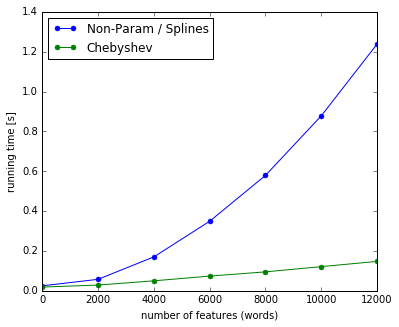
\includegraphics[width=5cm]{images/speed.png}
\caption{Plots of computational times w.r.t. the number of selected words in 20NEWS for non-parametric filters, spline-based filters \cite{art:HenaffBrunaLeCun15DLgraphs} and Chebyshev-based filters. The architecture is CN32+softmax with $K=5$ for splines and Chebyshev. We consider a mini-batch size of 100 data, and computations are carried out on an NVIDIA GPU K40c.}
\label{fig2}
\end{figure}







\noindent
Observe that non-parametric filters are most costly as they require $O(n)$ parameters to learn, and they are unable to learn localized filters, unlike \cite{art:HenaffBrunaLeCun15DLgraphs} and our model. This is particularly illustrated on Table \ref{tab6}, where non-parametric filters provide less accurate results. Besides, our model outperforms the classification accuracy of \cite{art:HenaffBrunaLeCun15DLgraphs} on MNIST.


\begin{table*}[h!]
 \centering
{\small
\begin{tabular}{|c|c|c|c|c|c|c|c|c|}
\hline
 Architecture & Accuracy  \\
\hline
CN10 (Non-Param filters) + softmax & 95.75 \\
CN10 (Spline filters)  + softmax & 97.26 \\
CN10 (Chebyshev filters)  + softmax & 97.48 \\
CN32-P4-CN64-P4-FC512-softmax  (Non-Param filters) & 96.28 \\
CN32-P4-CN64-P4-FC512-softmax  (Spline filters) & 97.15 \\
CN32-P4-CN64-P4-FC512-softmax  (Chebyshev filters) & 98.65 \\
\hline
\end{tabular}
}
\caption{Comparison of precisions between non-parametric filters, spline-based filters \cite{art:HenaffBrunaLeCun15DLgraphs} and Chebyshev-based filters [our model] on MNIST. For spline and Chebyshev filters, we picked $K=20$.} 
\label{tab6}
\end{table*}


\noindent
Eventually, we plot in Figure  \ref{fig1} the curves of accuracy and energy loss w.r.t. the number of iterations for the three types of filters. 


\begin{figure}[h!]
\centering
\subfigure[]{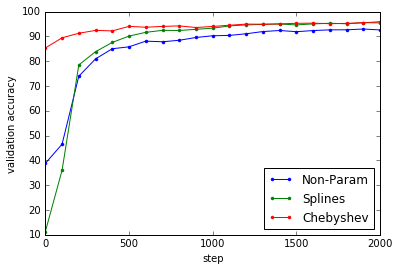
\includegraphics[width=6cm]{images/acc.png}}
\hspace{0.5cm}
\subfigure[]{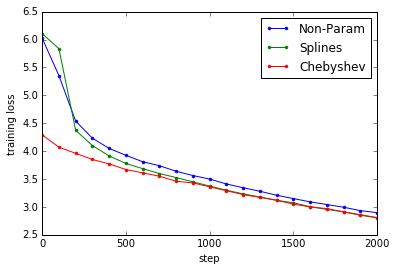
\includegraphics[width=6cm]{images/loss.png}}
\caption{Plots of accuracy (a) and energy loss (b) w.r.t. the number of iterations.}
\label{fig1}
\end{figure}



\section{Conclusion and Future Work}
\vspace{-0.2cm}
We have introduced an efficient implementation of CNNs on non-Euclidean manifolds represented by graphs using tools from SPG. Experiments have shown the ability of the model to extract the local stationary features through the graph convolutional layers. Future works will investigate two directions. First, we will explore applications of this generic model to important fields where the data naturally lie on non-artificially constructed graphs such as social networks, biological networks, or telecommunication networks. It makes actually more sense to apply this generalized CNN framework to natural network-based data, rather than artificially created networks which quality may vary as seen in the experiments. Second, we will also improve this framework with tools developed in SGP, including graph wavelet operators \cite{art:HammondVandergheynstGribonval11GraphWav,art:CoifmanLafon06DifMap,pro:GavishNadlerCoifman10GraphHaar,pro:ChenChengMallat14deepHaar,pro:RustamovGuibas14deepHaar}, spectral graph coarsening techniques \cite{art:ShumanFarajiVandergheynst16PyramTrans}, and improved localization properties \cite{pro:TsitsveroBarbarossa15Uncert,pro:PasdeloupAlamiGriponRabbat15Uncert,art:PerraudinRicaudShumanVandergheynst16Uncert}.












\newpage

%\vspace{-0.15cm} in .bbl
\bibliographystyle{plain}
{\setstretch{0}
{\small
%\bibliography{bib_nips16}
\bibliography{bib_nips16_short}
}
}




\end{document}















